\graphicspath{{05_analysis/figures/}} % Location of the graphics files

\chapter{Linguistic Analysis Based on Spatial Expressions}
\label{05_chp:analysis}

Recent models achieve promising results in visually grounded dialogues. However, existing datasets often contain undesirable biases and lack sophisticated linguistic analyses, which make it difficult to understand how well current models recognize their precise linguistic structures. To address this problem, we make two design choices: first, we focus on our OneCommon Corpus, which contains minimal bias by design. Second, we analyze their linguistic structures based on \textit{spatial expressions} and provide comprehensive and reliable annotation for 600 dialogues. We show that our annotation captures important linguistic structures including predicate-argument structure, modification and ellipsis. In our experiments, we assess our improved baseline's understanding of these structures through reference resolution (Chapter \ref{04_chp:interpretation}). We demonstrate that our annotation reveals both the strengths and weaknesses of our baseline in essential levels of detail. Overall, we propose a novel framework and resource for investigating fine-grained language understanding in visually grounded dialogues.

\section{Introduction}
\label{05_sec:introduction}

Visual dialogue is the task of holding natural, often goal-oriented conversation in a visual context \citep{das2017visual,de2017guesswhat}. This typically involves two types of advanced grounding: \textit{symbol grounding} \citep{harnad1990symbol}, which bridges symbolic natural language and continuous visual perception, and \textit{common grounding} \citep{clark1996using}, which refers to the process of developing mutual understandings through successive dialogues. As noted in \citet{monroe2017colors} and \citet{udagawa2019natural}, the \textit{continuous} nature of visual context introduces challenging symbol grounding of nuanced and pragmatic expressions. Some further incorporate \textit{partial observability} where the agents do not share the same context, which introduces complex misunderstandings and partial understandings that need to be resolved through advanced common grounding \citep{udagawa2019natural,haber-etal-2019-photobook}.

Despite the recent progress on these tasks, it remains unclear what types of linguistic structures can (or cannot) be properly recognized by existing models for two reasons. First, existing datasets often contain undesirable biases which make it possible to make correct predictions \textit{without} recognizing the precise linguistic structures \citep{goyal2017making,cirik-etal-2018-visual,agarwal-etal-2020-history}. Second, existing datasets severely lack in terms of sophisticated linguistic analysis, which makes it difficult to understand what types of linguistic structures exist or how they affect model performance.

To address this problem, we make the following design choices in this work:

\begin{itemize}%[leftmargin=1em] \setlength{\parskip}{0pt}
\item We focus on our OneCommon Corpus, a simple yet challenging collaborative reference task under continuous and partially-observable context. In this dataset, the visual contexts are kept simple and controllable to remove undesirable biases while enhancing linguistic variety. In total, 5,191 successful dialogues are fully annotated with referring expressions (called \textit{markables}) and their referents, which can be leveraged for further linguistic analysis.

\item To capture the linguistic structures in these dialogues, we propose to annotate \textit{spatial expressions} which play a central role in visually grounded dialogues. We take inspiration from the existing annotation frameworks \citep{pustejovsky2011iso,pustejovsky2011using,petruck-ellsworth-2018-representing,ulinski-etal-2019-spatialnet} but also make several simplifications and modifications to improve coverage, efficiency and reliability.\footnote{For instance, we define \textit{spatial expressions} in a broad sense and include spatial attributes (e.g. object size and color) as well as their comparisons.}
\end{itemize}

\begin{figure*}[t!]
\centering
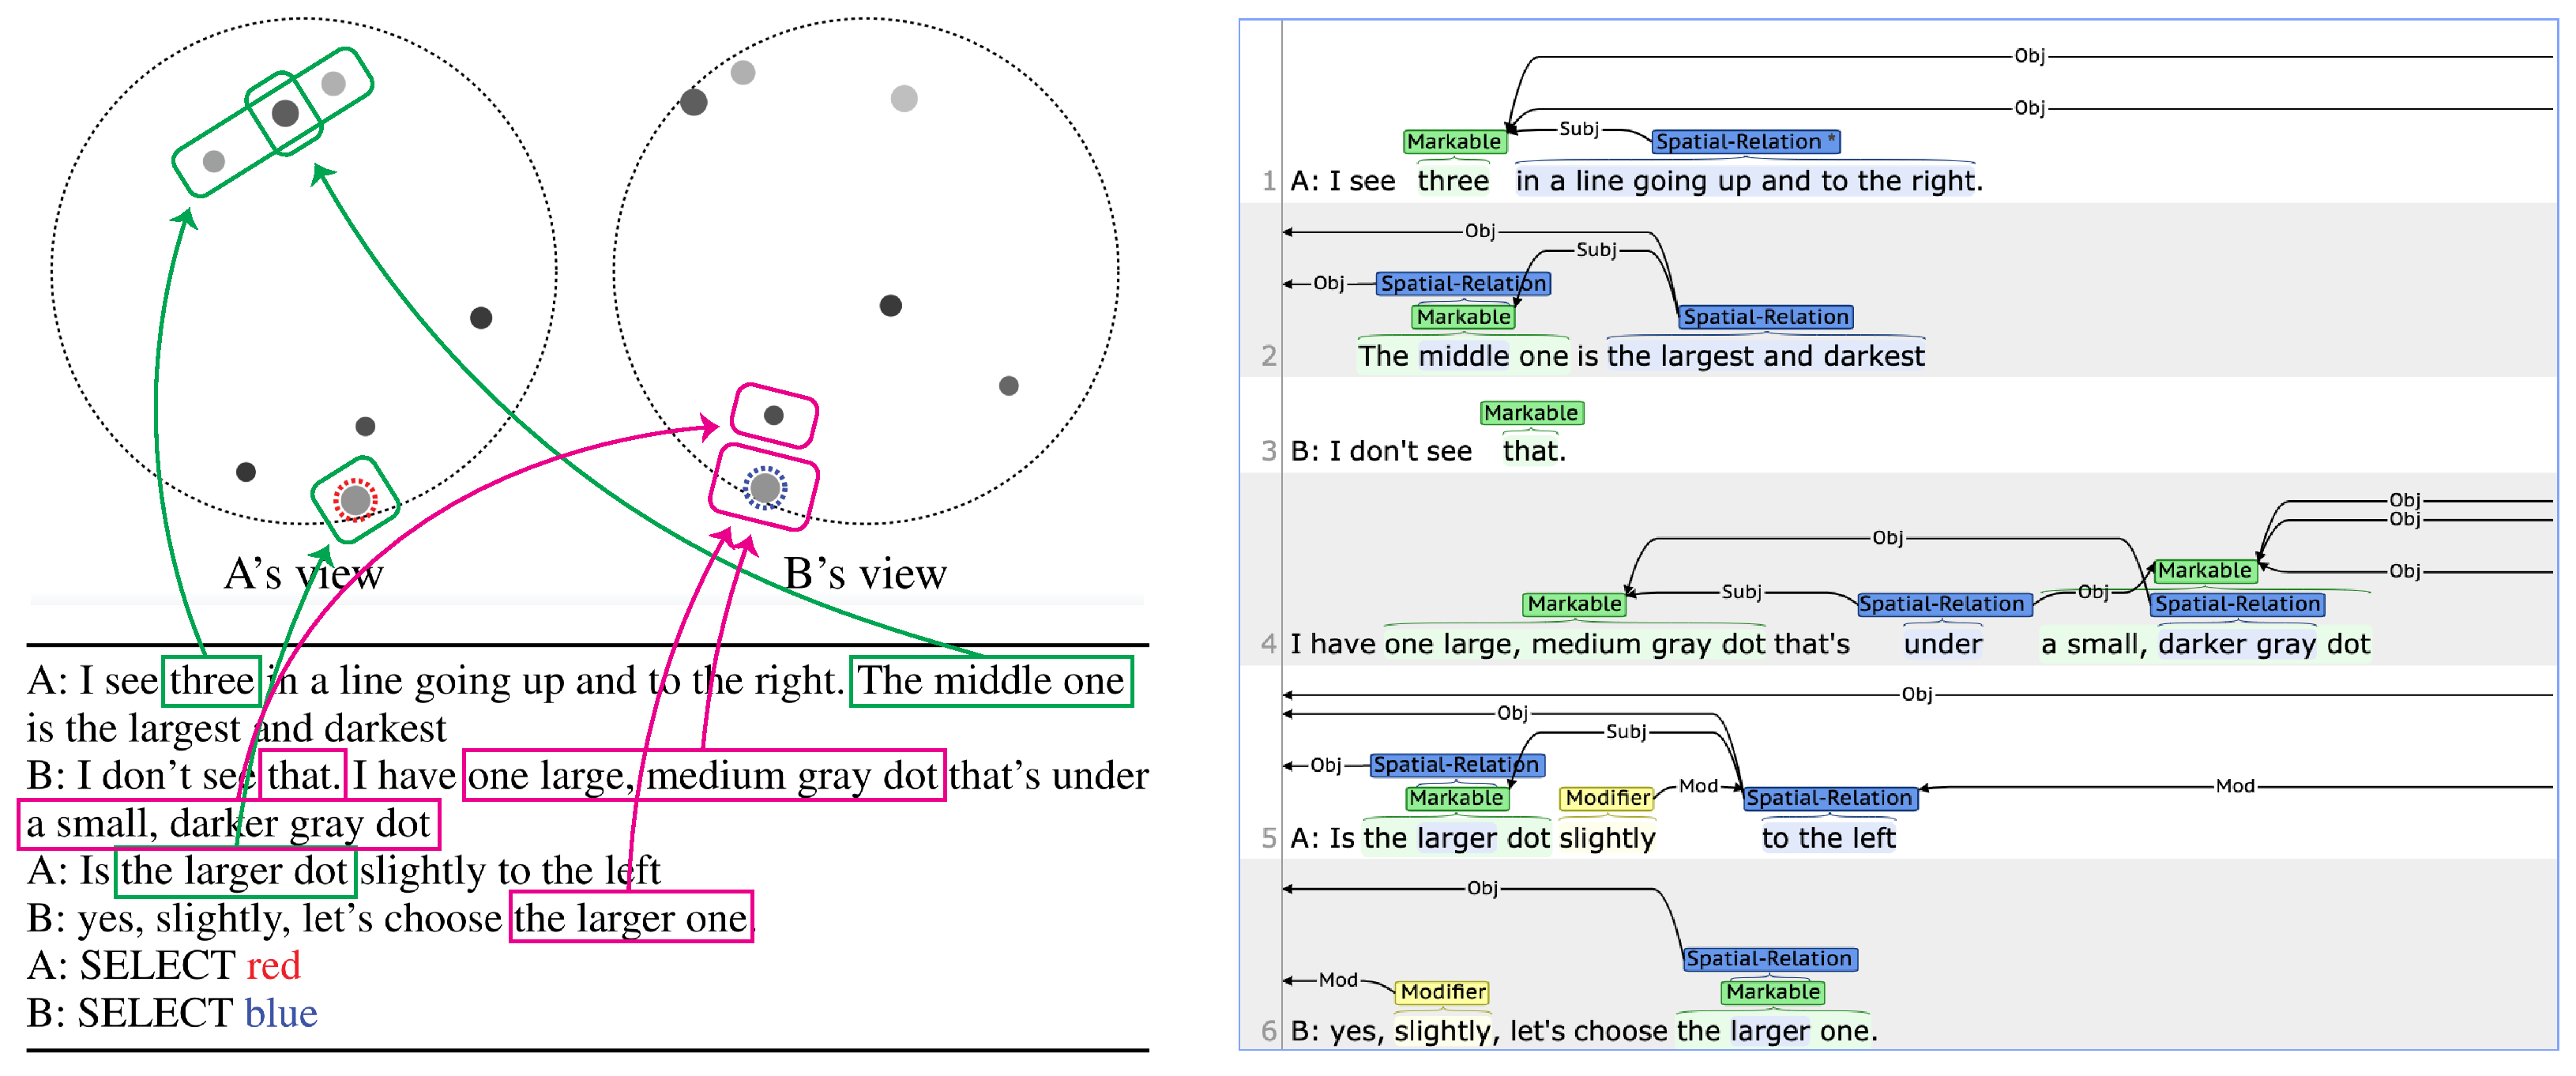
\includegraphics[width=\textwidth]{spatial_expression.pdf}
\caption{Example dialogue from OneCommon Corpus with reference resolution annotation (left) and our spatial expression annotation (right). We consider spatial expressions as predicates and annotate their arguments as well as modifiers.% For further details of the original dataset and our annotation schema, see Section \ref{sec:annotation}.
}
\label{05_fig:first_example}
\end{figure*}

As shown in Figure \ref{05_fig:first_example}, we consider spatial expressions as \textit{predicates} with existing markables as their \textit{arguments}. We distinguish the argument roles based on \textit{subjects} and \textit{objects}\footnote{Our \textit{subject}-\textit{object} distinction corresponds to other terminologies such as \textit{trajector}-\textit{landmark} or \textit{figure}-\textit{ground}.} and annotate \textit{modifications} based on nuanced expressions (such as ``slightly''). By allowing the arguments to be in previous utterances, our annotation also captures \textit{argument ellipsis} in a natural way.

In our experiments, we focus on reference resolution to study the model's comprehension of these linguistic structures. Since we found the existing baseline to perform relatively poorly (especially on the exact match rate), we propose a simple method of incorporating \textit{numerical constraints} in model predictions, which significantly improved its prediction quality.

Based on our annotation, we conduct a series of analyses to investigate whether the model predictions are \textit{consistent} with the spatial expressions. Our main finding is that the model is adept at recognizing entity-level attributes (such as color and size) but mostly fails in capturing inter-entity relations (especially placements): using the terminologies from \citet{landau1993and}, the model can recognize the \textit{what} but not the \textit{where} in spatial language. We also conduct further analyses to investigate the effect of other linguistic factors.

Overall, the contributions of this chapter are as follows:

\begin{itemize}
  \item We proposed a novel framework of annotating spatial expressions by leveraging referring expressions in visual dialogues.
  \item We sampled 600 random dialogues from OneCommon Corpus with reference resolution annotation (c.f. Chapter \ref{04_chp:interpretation}) and further conducted the annotation of spatial expressions.
  \item Our annotation captures important linguistic structures in visual dialogues, including predicate-argument structure, modification and ellipsis.
  \item Based on our improved baseline, we assess how well the end-to-end models can recognize the precise linguistic structures in the reference resolution task.
\end{itemize}


\section{Annotation Procedure}
\label{05_sec:annotation_procedure}

In this work, we randomly sample 600 dialogues from the annotated OneCommon Corpus (5,191 dialogues annotated with reference resolution) to conduct further annotation of spatial expressions. Our annotation procedure consists of three steps: \textit{spatial expression detection}, \textit{argument identification} and \textit{canonicalization}.
%Based on these annotation, we conduct fine-grained analyses of the dataset (Subsection \ref{subsec:annotation_results}) as well as the baseline models (Subsection \ref{subsec:model_analysis}). For further details and examples of our annotation, see Appendix \ref{sec:annotation_examples}.

\subsection{Step 1: Spatial Expression Detection}
\label{05_subsec:spatial_expression_detection}

Based on \citet{pustejovsky2011iso,pustejovsky2011using}, spatial expressions are defined as the ``constructions that make explicit reference to the spatial attributes of an object or spatial relations between objects''.\footnote{Note that their term \textit{object} corresponds to our term \textit{entity}.} We generally follow this definition and detect all spans of spatial attributes and relations in the dialogue. To make the distinction clear, we consider entity-level information (like color and size) as spatial attributes and other information (such as location and \textit{explicit} attribute comparison) as spatial relations. Spatial attributes could be annotated as adjectives (``dark''), prepositional phrases (``of light color'') or noun phrases (``a black dot''), while spatial relations could be adjectives (``lighter''), prepositions (``near''), and so on. We also detect the modification of spatial expressions based on negation and nuanced expressions, i.e. degree modifiers (c.f. Section \ref{03_subsec:difficulty_analysis}).

Although we allow certain flexibility in determining their spans, holistic/interdependent expressions (such as ``all shades of gray'', ``sloping up to the right'', ``very slightly'') were instructed to be annotated as a single span. Independent expressions (e.g. connected by conjunctions) could be annotated separately or jointly if they had the same structure (e.g. same arguments and modifiers).

For the sake of efficiency, we \underline{do not} annotate spatial attributes and their modifiers inside markables (see Figure \ref{05_fig:first_example}), since their spans and arguments are easy to be detected automatically.

\subsection{Step 2: Argument Identification}
\label{05_subsec:argument_identification}

Secondly, we consider the detected spatial expressions as \textit{predicates} and annotate referring expressions (markables) as their \textit{arguments}. This approach has several advantages: first, it has broad coverage since referring expressions are prevalent in visual dialogues. In addition, by leveraging \textit{exophoric} references which directly bridge natural language and the visual context, we can conduct essential analyses related to symbol grounding across the two modalities (c.f. Section \ref{02_sec:symbol_grounding}).

To be specific, we distinguish the argument roles based on subjects and objects. We allow arguments to be in previous utterances \textit{only if} they are unavailable in the present utterance. Multiple markables can be annotated for the subject/object roles, and no object need to be annotated in cases of spatial attributes, nominal/verbal expressions (``triangle'', ``clustered'') or \textit{implicit global objects} as in superlatives (``darkest (of all)''). If the arguments are indeterminable based on these roles (as in enumeration, e.g. ``\underline{From left to right}, there are ...''), they were marked as \textit{unannotatable}. Modificands of the modifiers (which could be either spatial attributes or relations) were also identified in this step. We show some illustrative examples in Figures \ref{05_fig:spatial_attribute}, \ref{05_fig:subject_ellipsis} and \ref{05_fig:unannotatable}.

\begin{figure}[t!]
\centering
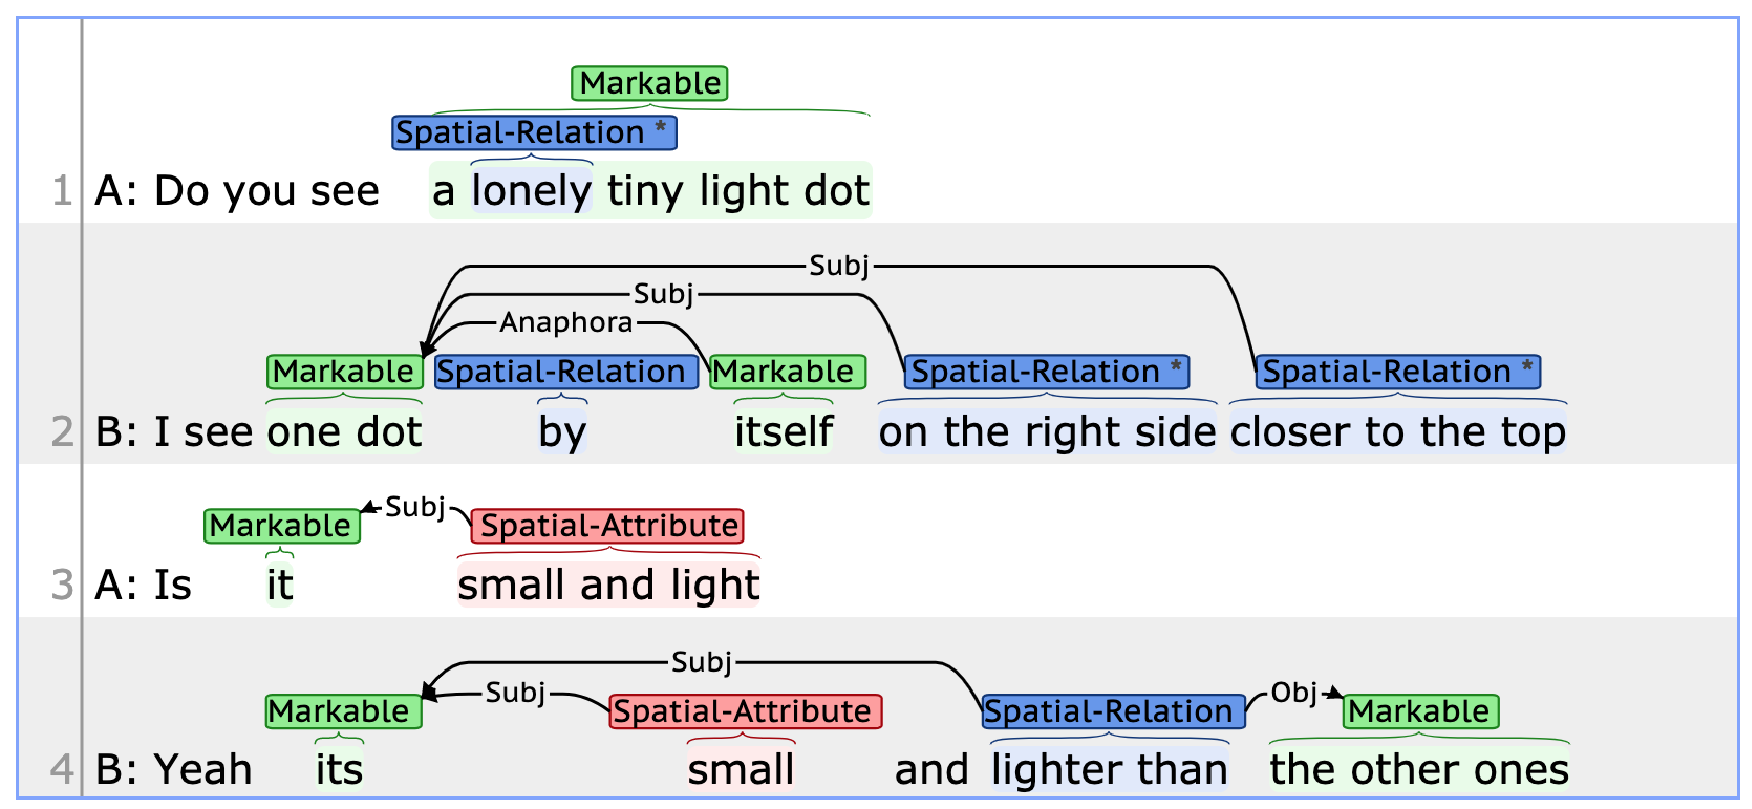
\includegraphics[width=0.6\columnwidth]{C_09b2a91332a64c12a3235d69a9e1f5da.pdf}
\caption{An example with spatial attributes (e.g. ``small and light'').}
\label{05_fig:spatial_attribute}
\end{figure}

\begin{figure}[t!]
\centering
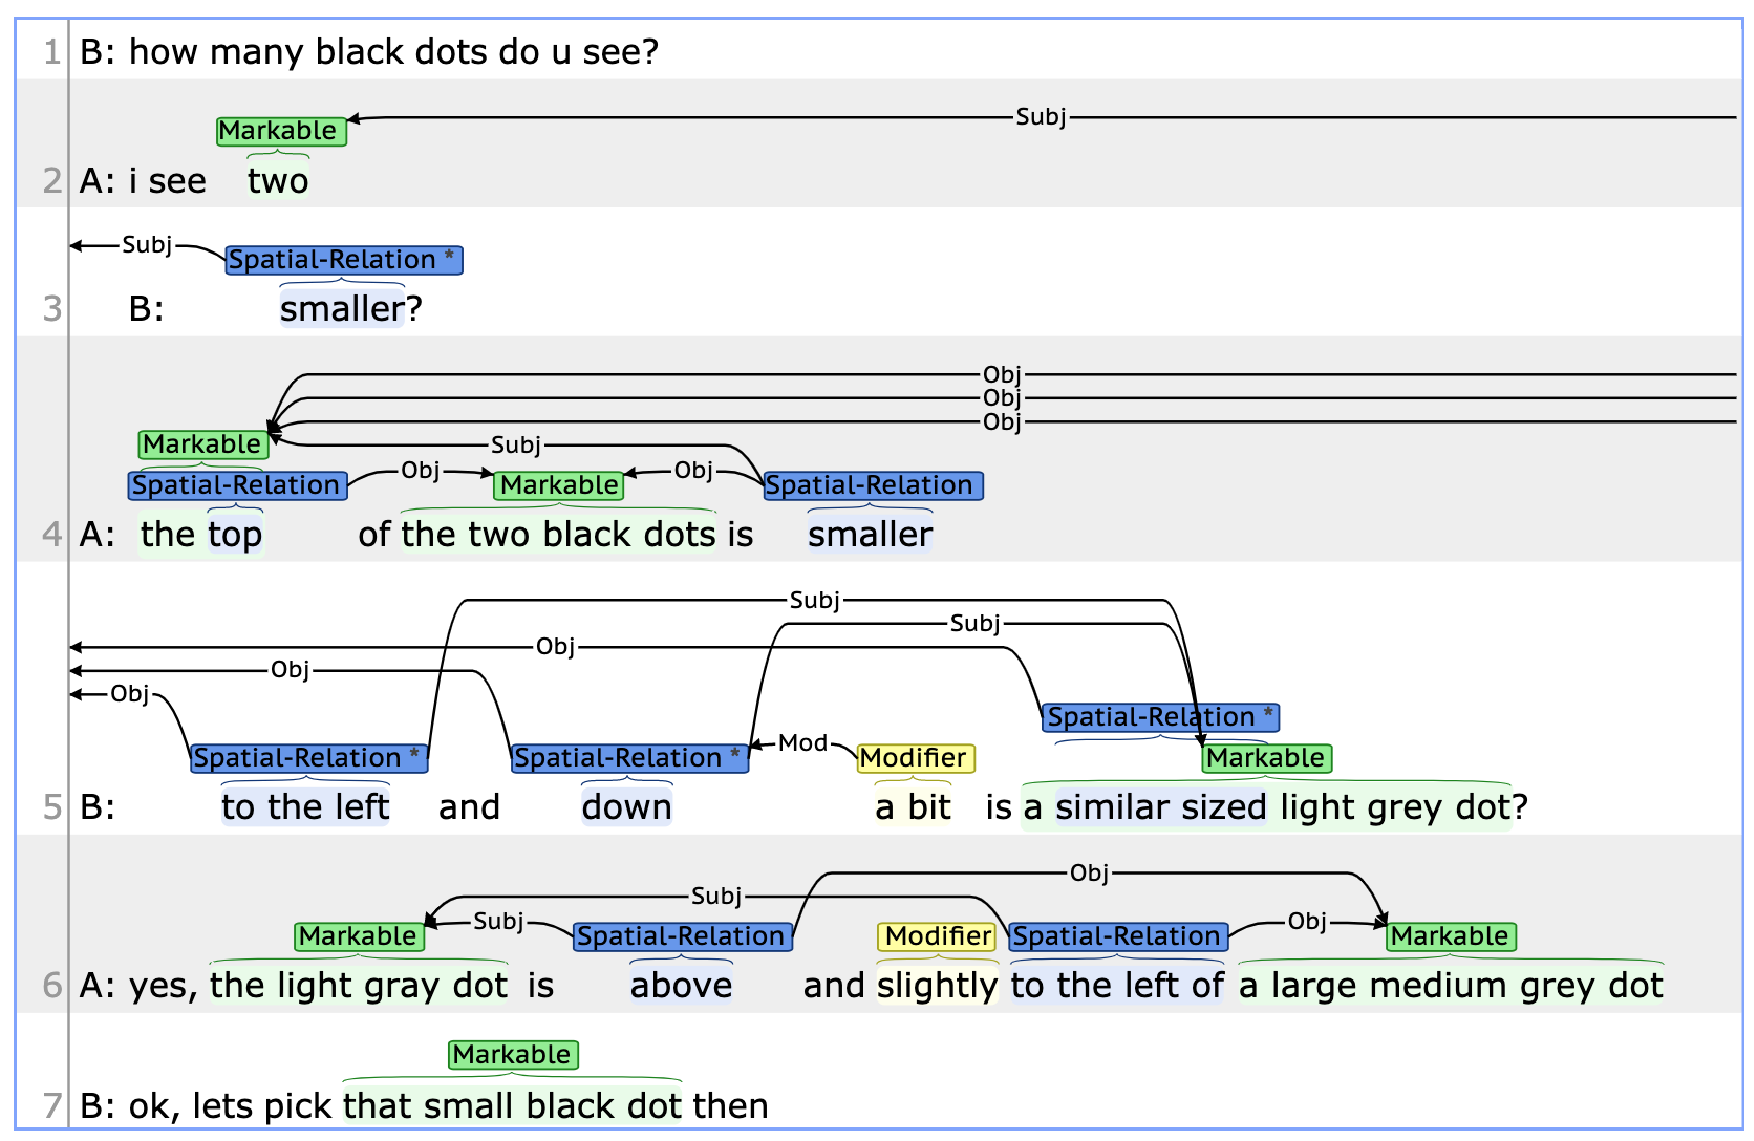
\includegraphics[width=0.6\columnwidth]{C_3bc6ee0e230445ab98661b03f6903ae5.pdf}
\caption{An example with subject ellipsis (``B: smaller?'').}
\label{05_fig:subject_ellipsis}
\end{figure}

\begin{figure}[t!]
\centering
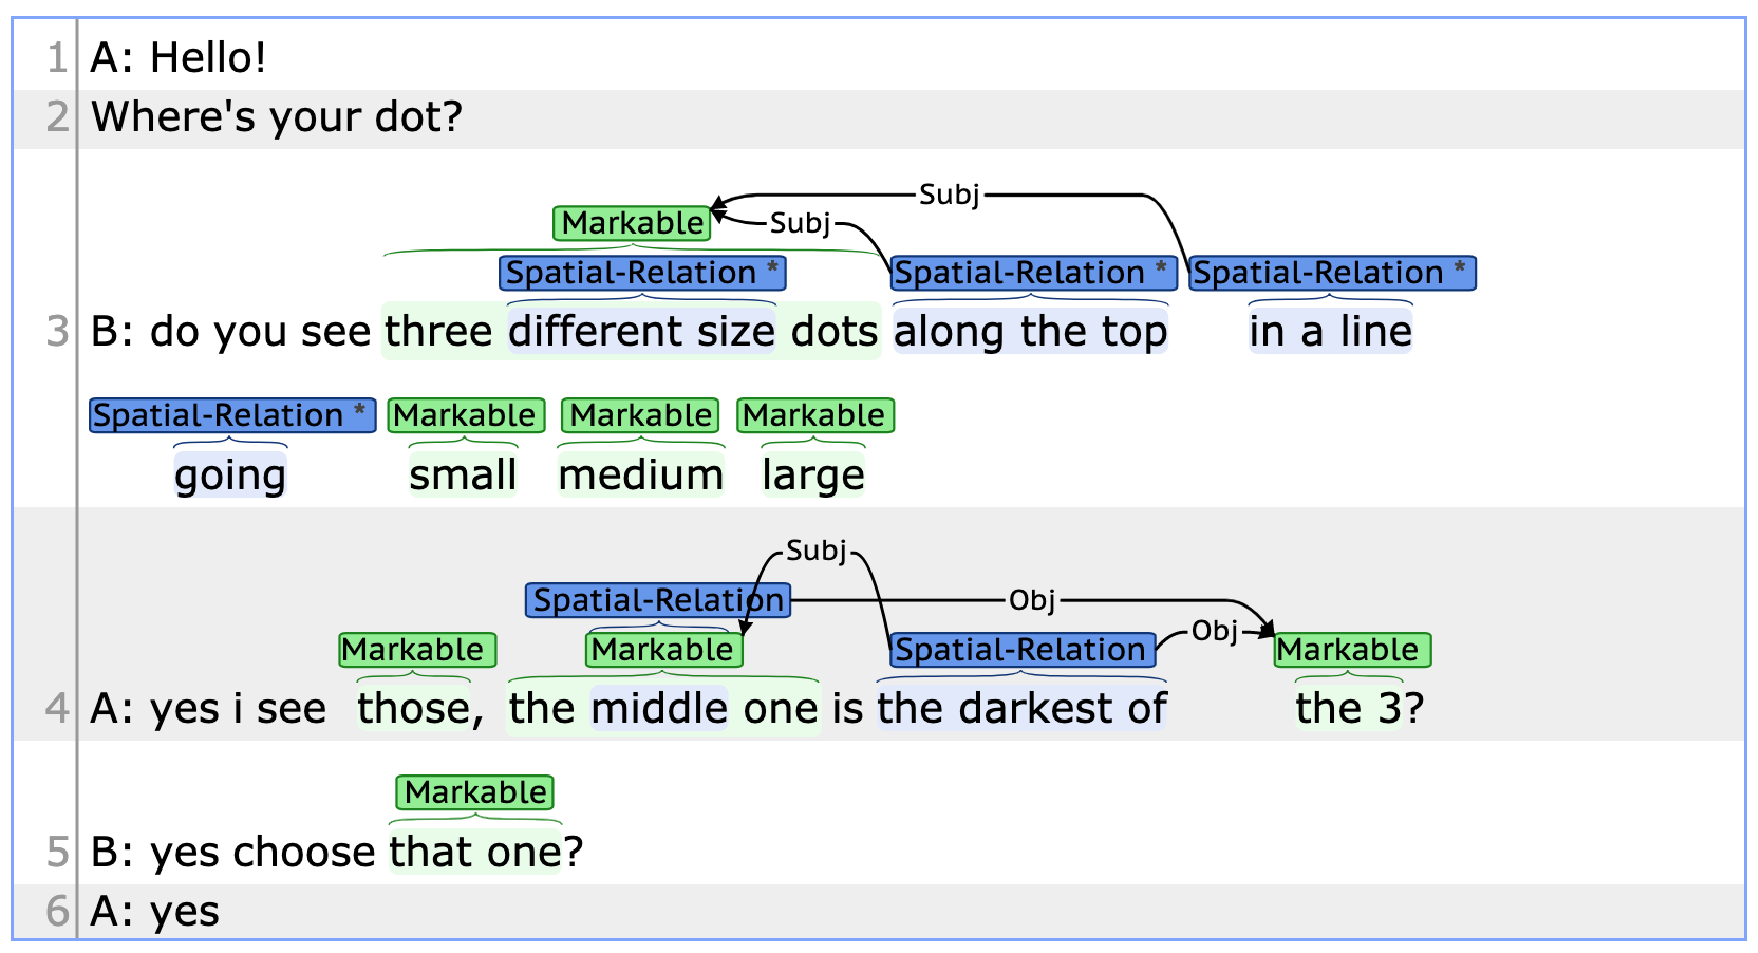
\includegraphics[width=0.6\columnwidth]{C_0e7e8399d1b64b598bcafa58976c05ac.pdf}
\caption{An example with unannotatable relation, ``going (small medium large)''.}
\label{05_fig:unannotatable}
\end{figure}

\subsection{Step 3: Canonicalization}
\label{05_subsec:canonicalization}

Finally, we conduct canonicalization of the spatial expressions and modifiers. Since developing a complete ontology for this domain is infeasible or too expensive, we focus on canonicalizing the central \textit{spatial relations} in this work: we \underline{do not} canonicalize spatial attributes manually since this can be conducted automatically (c.f. Section \ref{05_subsec:spatial_attributes}).

According to \citet{landau2017update}, there are 2 classes of relations in spatial language: \textit{functional} class whose core meanings engage force-dynamic relationship (such as \textit{on}, \textit{in}) and \textit{geometric} class whose core meanings engage geometry (such as \textit{left}, \textit{above}). Since functional relations are less common in this dataset and more difficult to define due to their vagueness and context dependence \citep{platonov2018computational}, we focus on the following 5 categories of geometric relations and attribute comparisons, including a total of 24 canonical relations which can be defined explicitly.

\begin{itemize}

\item \textbf{Direction} requires the subjects and objects to be placed in a certain orientation: \textit{left}, \textit{right}, \textit{above}, \textit{below}, \textit{horizontal}, \textit{vertical}, \textit{diagonal}.

\item \textbf{Proximity} is related to the distance between subjects, objects or other entities: \textit{near}, \textit{far}, \textit{alone}.

\item \textbf{Region} restricts the subjects to be in a certain region determined by the objects: \textit{interior}, \textit{exterior}.

\item \textbf{Color comparison} is related to the comparison of color among subjects and objects: \textit{lighter}, \textit{lightest}, \textit{darker}, \textit{darkest}, \textit{same color}, \textit{different color}.

\item \textbf{Size comparison} is related to the comparison of size among subjects and objects: \textit{smaller}, \textit{smallest}, \textit{larger}, \textit{largest}, \textit{same size}, \textit{different size}.

\end{itemize}

To be specific, we annotate whether each detected spatial relation \textit{implies} any of the 24 canonical relations. Each spatial relation can imply multiple canonical relations (e.g. ``on the upper right'' implies \textit{right} and \textit{above}) or none (e.g. ``(forming a) triangle'' does not imply any of the above relations).

In addition, we consider 6 modification types (the 5 degree modifiers from Figure \ref{03_fig:degree_modifiers} and \textit{negation}) and canonicalize each modifier into one type. For example, ``very slightly'' is considered to have the overall type of the \textit{diminisher}.


\section{Annotation Results}
\label{05_sec:annotation_results}

\subsection{Annotation Reliability}
\label{05_subsec:annotation_reliability}

\begin{table}[ht]
\centering \small
\setlength{\tabcolsep}{9pt}
\setlength{\aboverulesep}{0pt}
\setlength{\belowrulesep}{0pt}
\setlength{\extrarowheight}{.75ex}
\begin{tabular}{ll|cc}
\toprule
\multicolumn{2}{c|}{Annotation} & Agreement (\%) & Cohen's $\kappa$ \\
\midrule
\multirow{3}{*}{Span Detection} & Attribute & 98.5 & 0.88 \\
& Relation & 95.1 & 0.87 \\
& Modifier & 99.2 & 0.86 \\
\midrule
\multirow{3}{*}{\parbox{2cm}{Argument Identification}} & Subject & 98.8 & 0.96 \\
& Object & 95.9 & 0.79 \\
& Modificand & 99.6 & 0.98 \\
\midrule
\multirow{2}{*}{Canonicalization} & Relation & 99.7 & 0.96 \\
& Modifier & 87.5 & 0.83 \\
\bottomrule
\end{tabular}
\caption{
Results of our reliability analysis.
}
\label{05_tab:reliability_results}
\end{table}

To test the reliability of our annotation, two trained annotators (the authors) independently detected the spatial expressions and modifiers in 50 dialogues. Then, using the 50 dialogues from one of the annotators, two annotators independently conducted argument identification and canonicalization. We show the observed agreement and Cohen's $\kappa$ \citep{cohen1968weighted} in Table \ref{05_tab:reliability_results}.

For span detection, we computed the token level agreement of spatial expressions and modifiers. Despite having certain freedom for determining their spans, we observed high agreement in general (including their start/end positions).

For argument identification, we computed the exact match rate of the arguments and modificands. As a result, we observed near perfect agreement for subject/modificand identification. For object identification, the result was comparatively worse: however, upon further inspection, we verified that 73.5\% of the disagreements were essentially based on the same markables (e.g. coreferences).

Finally, we observed reasonably high agreement for relation/modifier canonicalization as well. Overall, we conclude that all steps of our annotation can be conducted with high reliability.

\subsection{Annotation Statistics}
\label{05_subsec:annotation_statistics}

\begin{table}[th]
\centering \small
\setlength{\tabcolsep}{9pt}
\begin{tabular}{lcc}
\toprule
 & Attribute & Relation \\
 \midrule
Total annotated & 378 & 4,300 \\
Average per dialogue & 0.63 & 7.17 \\
Unique expressions & 121 & 1,139 \\
Inter-utterance subject (\%) & 1.59 & 1.37 \\
Inter-utterance object (\%) & - & 14.65 \\
No object (\%) & - & 30.84 \\
Unannotatable (\%) & 0.79 & 0.79 \\
\midrule
Modified (\%) & 36.51 & 16.86 \\
\phantom{----}-- Diminisher & 1.06 & 8.12 \\
\phantom{----}-- Moderator & 19.31 & 0.67 \\
\phantom{----}-- Booster & 9.00 & 2.16 \\
\phantom{----}-- Approximator & 7.41 & 4.26 \\
\phantom{----}-- Maximizer & 0.27 & 1.40 \\
\phantom{----}-- Negation & 0.53 & 0.42 \\
\bottomrule
\end{tabular}
\caption{
Statistics of our spatial expression annotation in 600 random dialogues.
}
\label{05_tab:annotation_statistics}
\end{table}

The basic statistics of our annotation are summarized in Table \ref{05_tab:annotation_statistics}. Note that there are relatively few spatial attributes annotated, since most of them appeared inside the markables (hence not detected manually). However, a large number of spatial relations with non-obvious structures were identified.

In both expressions, we found over 1\% of the subjects and 14\% of the objects to be present only in previous utterances, which indicates that argument level ellipses are common and need to be resolved in visual dialogues. For spatial relations, about 30\% did not have any explicit objects.

Our annotation also verified that a large portion of the spatial expressions (37\% for spatial attributes and 17\% for relations) accompanied modifiers. In addition, we can see that \textit{neutrality} is the most common type of modification for spatial attributes (as in \textit{medium gray}, \textit{medium sized}), and \textit{subtlety} and \textit{uncertainty} to be the most common types for spatial relations. It is interesting to note that the frequencies of modification types vary significantly with spatial attributes and relations, except for \textit{negation}.

Finally, less than 1\% of spatial expressions were \textit{unannotatable} based on our schema, which verifies its broad coverage. Overall, our annotation can capture important linguistic structures of visually grounded dialogues, and it is straightforward to conduct even further analyses (e.g. by focusing on specific canonical relations or modifications).

\section{Model Refinement}
\label{05_sec:model_evaluation}


\subsection{Evaluation}
\label{05_subsec:evaluation}

In our experiments, we focus on the \textit{reference resolution task} in OneCommon Corpus. As we discussed in Chapter \ref{04_chp:interpretation}, this can be used for probing the model's understanding of the intermediate dialogue process. As illustrated in Figure \ref{05_fig:first_example} (left), the goal of the task is to predict the referents of each markable based on the \textit{speaker}'s perspective. To collect model predictions for all dialogues, we split the whole dataset into 10 equal-sized bins and use each bin as the test set in the 10 rounds of the experiments.

\subsection{Model Architecture}
\label{05_subsec:models}

\begin{figure}[ht]
\centering
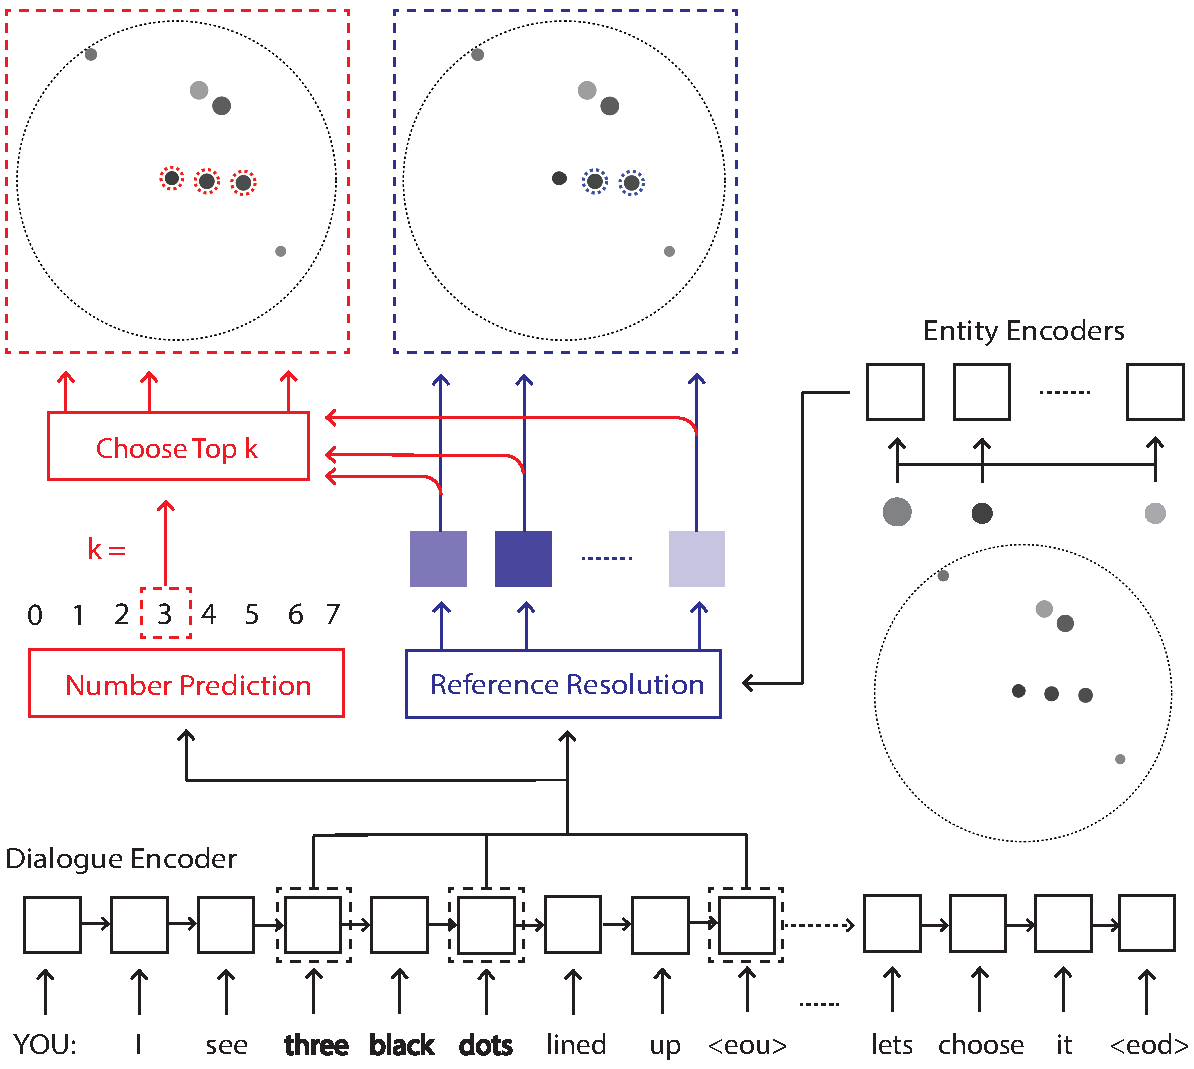
\includegraphics[width=0.7\columnwidth]{model_architecture.pdf}
\caption{Our model architecture. REF prediction flow is shown in blue and our NUMREF prediction flow in red.}
\label{05_fig:model_architecture}
\end{figure}

As a baseline, we use the \textit{REF} model from Chapter \ref{04_chp:interpretation}. As shown in Figure \ref{05_fig:model_architecture}, this model has two encoders: a \textit{dialogue encoder} based on a simple GRU \citep{cho2014properties} and a shared \textit{entity encoder} which outputs entity-level representation of the observation based on MLP and relational network \citep{santoro2017simple}. To predict the referents, REF takes the GRU's start position of the markable, end position of the markable and end position of the utterance to compute entity-level scores and judge whether each entity is a referent based on logistic regression.

However, since the predictions are made independently for each entity, this model often predicts the wrong number of referents, leading to low performance in terms of exact match rate. To address this issue, we trained a separate module to track the \textit{number} of referents in each markable. We formulate this as a simple classification task (between 0, 1, ..., 7) which can be predicted reliably with an average accuracy of $92$\%. Based on this module's prediction $k$, we simply take the top $k$ entities with the highest scores as the referents. We refer to this numerically constrained model as NUMREF.

Furthermore, we conduct feature level ablations to study the importance of each feature: for instance, we remove the xy-values from the structured input to ablate the \textit{location} feature.

\subsection{Results}
\label{05_subsec:reference_resolution_results}

\begin{table}[ht]
\centering \small
\setlength{\tabcolsep}{9pt}
\begin{tabular}{lcc}
\toprule
 & Entity-Level & Markable-Level \\
 & Accuracy (\%) & Exact Match (\%) \\
\midrule
REF & 85.71$\pm$0.23 & 33.15{\scriptsize $\pm$1.00} \\
\phantom{NN}$-$ location & 84.28{\scriptsize $\pm$0.27} & 30.53{\scriptsize $\pm$0.84} \\
\phantom{NN}$-$ color & 83.08{\scriptsize $\pm$0.32} & 17.09{\scriptsize $\pm$1.04} \\
\phantom{NN}$-$ size & 83.50{\scriptsize $\pm$0.22} & 19.41{\scriptsize $\pm$0.98} \\
\midrule
NUMREF & \textbf{86.03{\scriptsize $\pm$0.33}} & \textbf{54.94{\scriptsize $\pm$0.76}} \\
\phantom{NN}$-$ location & 83.35{\scriptsize $\pm$0.26} & 49.77{\scriptsize $\pm$0.64} \\
\phantom{NN}$-$ color & 81.19{\scriptsize $\pm$0.41} & 39.74{\scriptsize $\pm$1.31} \\
\phantom{NN}$-$ size & 82.39{\scriptsize $\pm$0.20} & 43.40{\scriptsize $\pm$0.67} \\
\midrule
Human & 96.26 & 86.90 \\
\bottomrule
\end{tabular}
\caption{
Results for the reference resolution task.
}
\label{05_tab:experiment_results}
\end{table}

We report the mean and standard deviation of the entity-level accuracy and markable-level exact match rate in Table \ref{05_tab:experiment_results}. Compared to REF, our NUMREF model slightly improves the entity-level accuracy and significantly outperforms it in terms of exact match rate, which validates our motivation. From the ablation studies, we can see that all features contribute to the overall performance, but color and size seem to have the largest impact. 

However, it remains difficult to see how and where these models struggle based on mere accuracy. For further investigation, we need more sophisticated \textit{behavioral testing} (black-box testing) to verify whether each model has the capability of recognizing certain concepts or linguistic structures \citep{ribeiro-etal-2020-beyond}.

\section{Model Analysis}
\label{05_sec:model_analysis}

To study the current model's strengths and weaknesses in detail, we investigate whether their predictions are \textit{consistent} with the central spatial expressions.

\subsection{Spatial Attributes}
\label{05_subsec:spatial_attributes}

\begin{figure}[ht]
\centering
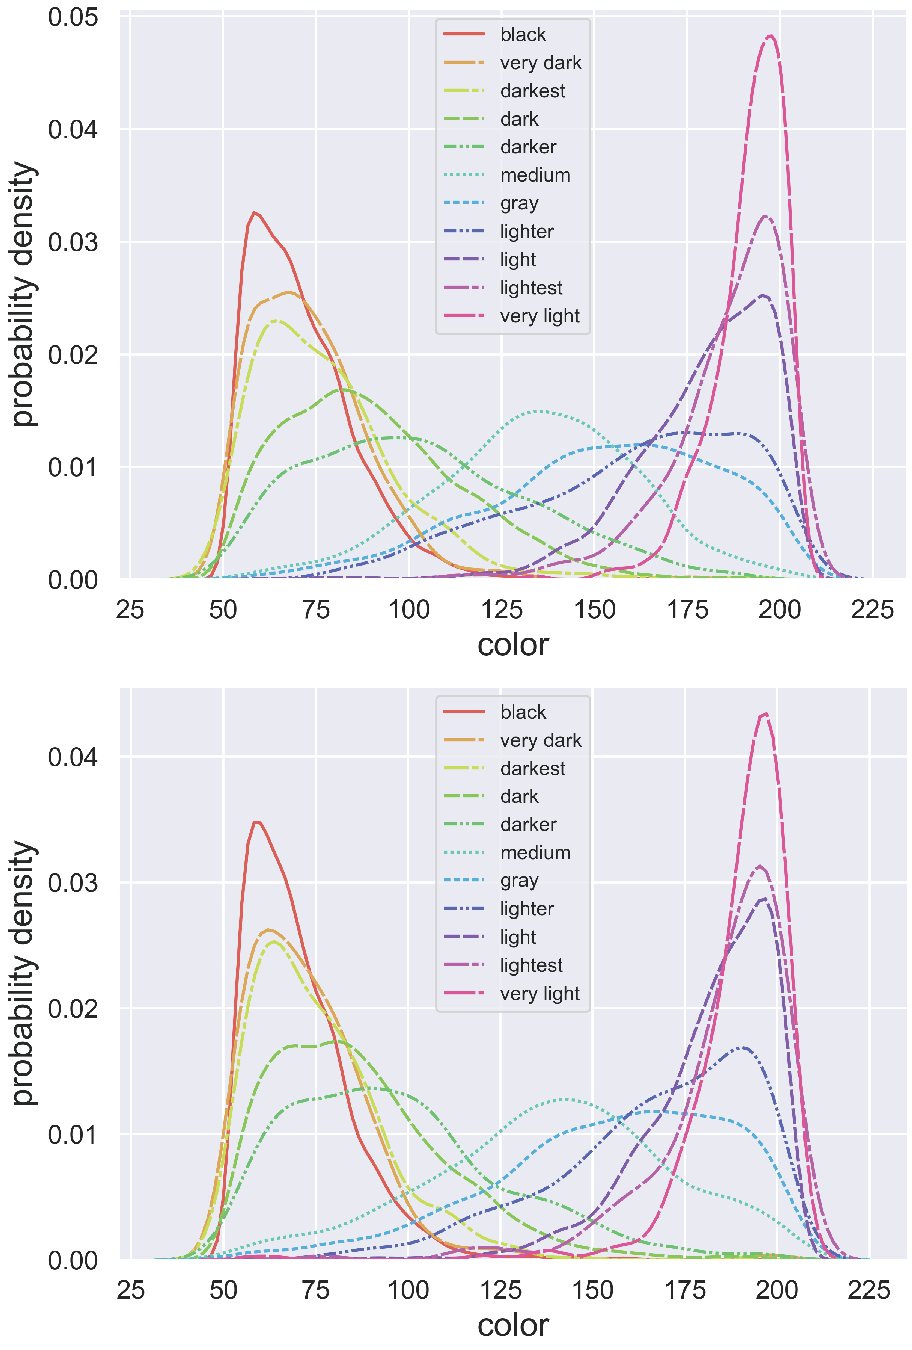
\includegraphics[width=0.6\columnwidth]{referent_color.pdf}
\caption{Referent color distributions. Top is human, bottom is NUMREF (smaller is darker in color axis).}
\label{05_fig:referent_color}
\end{figure}

First, we analyze whether the model predictions are consistent with the entity-level spatial attributes. Since most of them were confirmed to appear inside the markables (Section \ref{05_sec:annotation_results}), we automatically detect the expressions of \textit{color} in the markables, plot the distributions of the actual referent color, and compare the results between gold human annotation and model predictions (Figure \ref{05_fig:referent_color}).

From the figure, we can verify that the two distributions look almost identical for the common color expressions, and our NUMREF model seems to capture important characteristics of pragmatic expressions (same expression being used for wide range of colors) and modifications such as neutrality (\textit{medium}) and extremity (\textit{very dark}, \textit{very light}).\footnote{Spatial attributes with diminishers (such as \textit{slightly dark}) were relatively rare and omitted in the figure.} Note that we observed very similar results with the \textit{size} distributions as well.

Based on these results, we argue that the current model can capture entity-level attributes very well, including basic modification.

\subsection{Spatial Relations}
\label{05_subsec:spatial_relations}

\begin{table*}[th]
\centering \scalebox{0.77}{
\small
\def\arraystretch{1.0}
\newcommand{\intermidrule}{\cmidrule{2-13}}  
\setlength{\tabcolsep}{4pt}
\setlength{\aboverulesep}{0pt}
\setlength{\belowrulesep}{0pt}
\setlength{\extrarowheight}{.75ex}
\begin{tabular}{lcc|cacacacaca}
\toprule
\multicolumn{3}{c}{Models} & \multicolumn{2}{c}{REF} & \multicolumn{2}{c}{REF-abl} & \multicolumn{2}{c}{NUMREF} & \multicolumn{2}{c}{NUMREF-abl} & \multicolumn{2}{c}{Human} \\
\midrule
Category & Relation & \# Cases  & satisfy & \phantom{.}valid\phantom{.} & satisfy & \phantom{.}valid\phantom{.} & satisfy & \phantom{.}valid\phantom{.} & satisfy & \phantom{.}valid\phantom{.} & satisfy & \phantom{.}valid\phantom{.} \\
\midrule
\multirow{8}{*}{Direction}\phantom{..} & \textit{left} & 412 & 23.5 & 32.3 & 21.1 & 28.9 & \textbf{67.0} & \textbf{99.5} & 62.4 & \textbf{99.5} & 95.9 & 97.6 \\
 & \textit{right} & 468 & 28.0 & 35.5 & 24.6 & 30.8 & 67.3 & \textbf{98.7} & \textbf{68.2} & \textbf{98.7} & 95.3 & 96.4 \\
 & \textit{above} & 514 & 28.6 & 37.4 & 24.7 & 33.1 & 65.2 & 99.2 & \textbf{66.5} & \textbf{99.4} & 96.7 & 98.6 \\
 & \textit{below} & 444 & 25.2 & 34.5 & 21.6 & 27.9 & \textbf{66.0} & \textbf{99.1} & 62.2 & \textbf{99.1} & 96.4 & 96.8 \\
 & \textit{horizontal} & 37 & 54.1 & 70.3 & 27.0 & 59.5 & \textbf{59.5} & \textbf{100.0} & 51.4 & 97.3 & 91.9 & 100.0 \\
 & \textit{vertical} & 46 & 37.0 & 73.9 & 23.9 & 54.3 & 43.5 & \textbf{95.7} & \textbf{45.7} & \textbf{95.7} & 82.6 & 100.0 \\
 & \textit{diagonal} & 50 & 48.0 & 74.0 & 30.0 & 50.0 & \textbf{60.0} & \textbf{98.0} & \textbf{60.0} & \textbf{98.0} & 90.0 & 100.0 \\
\intermidrule
 & All & 1,971 & 27.8 & 37.6 & 23.4 & 31.9 & \textbf{65.5} & \textbf{99.0} & 64.1 & \textbf{99.0} & 95.5 & 97.6 \\
\midrule
\multirow{4}{*}{Proximity} & \textit{near} & 271 & 49.4 & 61.3 & 29.9 & 49.1 & \textbf{77.1} & 94.5 & 56.1 & \textbf{95.2} & 95.2 & 96.7 \\
 & \textit{far} & 27 & 29.6 & 40.7 & 33.3 & 40.7 & 77.8 & \textbf{100.0} & \textbf{92.6} & \textbf{100.0} & 96.3 & 96.3 \\
 & \textit{alone} & 111 & 36.9 & 44.1 & 45.0 & 54.1 & \textbf{68.5} & \textbf{94.6} & 67.6 &\textbf{94.6} & 91.9 & 94.6 \\
\intermidrule
 & All & 409 & 44.7 & 55.3 & 34.2 & 49.9 & \textbf{74.8} & 94.9 & 61.6 & \textbf{95.4} & 94.4 & 96.1 \\
\midrule
\multirow{3}{*}{Region} & \textit{interior} & 135 & 38.5 & 52.6 & 27.4 & 39.3 & \textbf{62.2} & 93.3 & 58.5 & \textbf{94.1} & 96.3 & 100.0 \\
 & \textit{exterior} & 62 & 40.3 & 48.4 & 40.3 & 53.2 & 80.6 & \textbf{98.4} & \textbf{87.1} & \textbf{98.4} & 98.4 & 98.4 \\
\intermidrule
 & All & 197 & 39.1 & 51.3 & 31.5 & 43.7 & \textbf{68.0} & 94.9 & 67.5 & \textbf{95.4} & 97.0 & 99.5 \\
\midrule
\multirow{7}{*}{Color} & \textit{lighter} & 147 & 23.1 & 25.9 & 6.8 & 8.2 & \textbf{84.4} & \textbf{100.0} & 57.1 & 99.3 & 97.3 & 98.0 \\
 & \textit{lightest} & 42 & 45.2 & 66.7 & 14.3 & 33.3 & \textbf{61.9} & \textbf{100.0} & 31.0 & \textbf{100.0} & 83.3 & 100.0 \\
 & \textit{darker} & 171 & 24.0 & 26.3 & 7.0 & 10.5 & \textbf{83.0} & \textbf{99.4} & 53.2 & \textbf{99.4} & 95.9 & 98.8 \\
 & \textit{darkest} & 48 & 56.2 & 64.6 & 14.6 & 33.3 & \textbf{66.7} & \textbf{100.0} & 35.4 & \textbf{100.0} & 89.6 & 97.9 \\
 & \textit{same} & 50 & 12.0 & 30.0 & 8.0 & 30.0 & \textbf{40.0} & \textbf{88.0} & 32.0 & 86.0 & 92.0 & 96.0 \\
 & \textit{different} & 14 & 64.3 & 71.4 & 71.4 & 71.4 & 64.3 & \textbf{100.0} & \textbf{78.6} & 92.9 & 92.9 & 100.0 \\
\intermidrule
 & All & 472 & 28.8 & 35.4 & 10.4 & 18.0 & \textbf{74.8} & \textbf{98.5} & 49.2 & 97.9 & 94.1 & 98.3 \\
\midrule
\multirow{7}{*}{Size} & \textit{smaller} & 213 & 27.7 & 31.5 & 7.5 & 9.9 & \textbf{80.8} & \textbf{100.0} & 59.6 & \textbf{100.0} & 98.6 & 99.5 \\
 & \textit{smallest} & 52 & 71.2 & 73.1 & 21.2 & 34.6 & \textbf{86.5} & \textbf{98.1} & 48.1 & \textbf{98.1} & 92.3 & 98.1 \\
 & \textit{larger} & 238 & 23.1 & 28.6 & 9.7 & 16.0 & \textbf{73.5} & \textbf{99.6} & 48.7 & \textbf{99.6} & 98.3 & 98.3 \\
 & \textit{largest} & 61 & 52.5 & 60.7 & 11.5 & 24.6 & \textbf{73.8} & \textbf{100.0} & 39.3 & \textbf{100.0} & 96.7 & 100.0 \\
 & \textit{same} & 103 & 34.0 & 42.7 & 18.4 & 27.2 & \textbf{80.6} & 88.3 & 65.0 & \textbf{91.3} & 98.1 & 100.0 \\
 & \textit{different} & 12 & 75.0 & 75.0 & 66.7 & 66.7 & \textbf{91.7} & \textbf{91.7} & 83.3 & 83.3 & 91.7 & 91.7 \\
\intermidrule
 & All & 679 & 33.4 & 38.7 & 12.4 & 18.9 & \textbf{78.2} & 97.8 & 54.3 & \textbf{98.1} & 97.6 & 99.0 \\
\bottomrule
\end{tabular}
}
\caption{
Canonical relation test results. We compute the \textit{satisfy} and \textit{valid} rate of the predictions for each canonical relation. Best scores of the models are in bold (-abl shows the corresponding feature ablated results).
}
\label{05_tab:satisfication_result}
\end{table*}

Next, we investigate whether the model predictions are consistent with the central spatial relations. Based on our annotation (Section \ref{05_sec:annotation_procedure}), we conduct simple tests to check whether the predicted referents satisfy each canonical relation. To be specific, our tests check for two conditions: whether the predictions are \textit{valid} (satisfy the minimal requirements, e.g. at least 2 referents predicted for \textit{near} relation), and if they are valid, whether the predictions actually \textit{satisfy} the canonical relation (e.g. referents are closer than a certain threshold).

Algorithm \ref{alg:left} shows our test for the canonical \textit{left} relation. Note that if no objects were annotated, we simply test whether the subject referents are on the left side of the player's view ($ mean(\mathcal{S}.x) < 0 $).

\begin{algorithm}[h]
\small
\DontPrintSemicolon
\SetAlgoNoEnd

\KwIn{subject referents $\mathcal{S}$, object referents $\mathcal{O}$, boolean $no\_object$}
\KwOut{boolean $satisfy$, boolean $valid$}
\If{$no\_object$}{
	$valid \leftarrow |\mathcal{S}| \! > \! 0$\\
	$satisfy \leftarrow valid \, \wedge \, mean(\mathcal{S}.x) \! < \! 0$
}\Else{
	$valid \leftarrow |\mathcal{S}| \! > \! 0 \, \wedge \, |\mathcal{O}| \! > \! 0$\\
	$satisfy \leftarrow valid \, \wedge \, mean(\mathcal{S}.x) \! < \! mean(\mathcal{O}.x)$
}
\Return $satisfy$, $valid$
\caption{Test for \textit{left} relation}
\label{alg:left}
\end{algorithm}

The results of our tests are summarized in Table \ref{05_tab:satisfication_result}. We also compare with the feature ablated models to estimate the test cases which can be satisfied \textit{without} using the corresponding features, i.e. location for \textit{direction}/\textit{proximity}/\textit{region} categories, color for \textit{color comparison}, and size for \textit{size comparison}.

First, we can verify that human annotation passes most of our tests, which is an important evidence of the reliability of our annotations and behavioral tests. We also confirmed that REF models often make \textit{invalid} predictions with overall poor performance, which is consistent with our expectation.

In \textit{direction}, \textit{proximity} and \textit{region} categories, we found that NUMREF model performs on par or only marginally better than its ablated version (and even underperforms it for simple relations like \textit{right} and \textit{above}): these results indicate that current model is still incapable of leveraging locational features to make more consistent predictions.\footnote{For relations like \textit{far} and \textit{different color}, ablated model may be better simply because referents tend to be more distant/dissimilar when predictions are closer to random.}

In \textit{color/size comparison}, NUMREF performs reasonably well, outperforming all other models: this indicates that the model can not only capture but also \textit{compare} entity-level attributes to a certain extent. However, there is still room left for improvement in almost all relations. It is also worth noting that \textit{size comparison} may be easier, as the range of size is limited (only \textit{6} compared to \textit{150} for color).

Overall, we conclude that current models still struggle in capturing most of the inter-entity relations, especially those related to placements.

\subsection{Further Analyses}
\label{05_subsec:further_analyses}

\begin{table}[h!]
\centering \small
\begin{tabular}{lccc}
\toprule
Linguistic Factors & \# Cases & NUMREF & Human  \\
 \midrule
Strong modification & 149 & 76.51 & 95.97 \\
Neutral & 3,094 & 70.46 & 95.77 \\
Weak modification & 490 & 66.12 & 95.10 \\
\midrule
Inter-utterance subject & 14 & 57.14 & 92.86 \\
Inter-utterance object & 265 & 72.08 & 94.72 \\
No object & 1,127 & 74.45 & 92.99 \\
Ignorable object & 1,805 & 69.64 & 97.23 \\
Unignorable object & 796 & 65.33 & 96.11 \\
\midrule
All & 3,728 & 70.17 & 95.71 \\
\bottomrule
\end{tabular}
\caption{
Satisfy rates classified by linguistic factors.
}
\label{further comparison}
\end{table}

Finally, we conduct further analyses to study other linguistic factors that affect model performance. Table \ref{further comparison} shows the results of our relation tests classified by notable linguistic structures.

In terms of modification, we can confirm that human performance is consistently high, while the model performs best for strong modification (modified by \textit{boosters} or \textit{maximizers}), decently for neutrals (\textit{moderators} or no modification), and worst on weak modification (\textit{diminishers} or \textit{approximators}). This indicates that large, conspicuous features are easier for the model to capture compared to small or more ambiguous features.

In terms of subject/object properties, human performance is also consistently high. In contrast, model performance is significantly worse for subject ellipsis (\textit{inter-utterance subject}), while remaining high for object ellipsis and \textit{no object} cases.

We also hypothesize that a large portion of the relations can actually be satisfied \textit{without} considering the objects, e.g. by simply predicting very dark dots as the subjects when the relation is \textit{darker} or \textit{darkest}. To distinguish such easy cases, we consider a relation as \textit{ignorable object} if the relation can be satisfied even if we ignore the objects (i.e. remove all object relations) based on gold referents. Our result verifies that there are indeed many cases of \textit{ignorable object}, and they seem slightly easier for the model to satisfy.

\begin{table}[h!]
\centering \small
\def\arraystretch{1.0}
\newcommand{\intermidrule}{\cmidrule{2-13}}  
\setlength{\tabcolsep}{4pt}
\setlength{\aboverulesep}{0pt}
\setlength{\belowrulesep}{0pt}
\setlength{\extrarowheight}{.75ex}
\begin{tabular}{lccaca}
\toprule
\multicolumn{2}{c}{Models} & \multicolumn{2}{c}{NUMREF} & \multicolumn{2}{c}{Human} \\
\midrule
value & mod-type & diff. & \# valid & diff. & \# valid \\
\midrule
\multirow{3}{*}{xy-value} & strong & 86.06 & 39 & 89.15 & 37 \\
& neutral & 80.92 & 1,586 & 73.52 & 1,558\\
& weak & 80.35 & 200 & 53.53 & 198 \\
\midrule
\multirow{3}{*}{color} & strong & 66.23 & 15 & 91.80 & 15 \\
& neutral & 56.98 & 234 & 60.14 & 232\\
& weak & 37.73 & 68 & 28.55 & 66 \\
\midrule
\multirow{3}{*}{size} & strong & 3.60 & 8 & 4.29 & 8 \\
& neutral & 2.67 & 337 & 2.70 & 320\\
& weak & 1.95 & 105 & 1.58 & 104 \\
\bottomrule
\end{tabular}
\caption{
Absolute differences of feature values in comparative relations (number of valid predictions shown in shade).
}
\label{05_tab:difference_comparison}
\end{table}

In Table \ref{05_tab:difference_comparison}, we study the effect of modification based on the  \textit{absolute difference} between subject and object features in comparative relations.\footnote{\textit{Left/right} for x-value, \textit{above/below} for y-value, \textit{lighter/darker} for color and \textit{smaller/larger} for size.}

In human annotation, the absolute difference naturally increases as the modification gets stronger. While model predictions also show this tendency, their results seem less sensitive to modification (particularly for locational features, i.e. xy-value) and may not be reflecting their full effect.

\section{Related Work}
\label{05_sec:related_work}

Linguistic structure plays a critical role in dialogue research. From theoretical aspects, various dialogue structures have been studied, including discourse structure \citep{stent-2000-rhetorical,asher2003logics}, speech act \citep{austin1962things,searle1969speech} and common grounding \citep{clark1996using,lascarides2009agreement}. In dialogue system engineering, various linguistic structures have been considered and applied, including syntactic dependency \citep{davidson-etal-2019-dependency}, predicate-argument structure \citep{yoshino2011spoken}, ellipsis \citep{quan-etal-2019-gecor,hansen2020you}, intent recognition \citep{silva2011symbolic,shi-etal-2016-deep}, semantic representation/parsing \citep{mesnil2013investigation,gupta-etal-2018-semantic} and frame-based dialogue state tracking \citep{williams2016dialog,elasri2017frames}. However, most prior work focus on dialogues where information is not grounded in external, perceptual modality such as vision. In this work, we propose an effective method of analyzing linguistic structures in visually grounded dialogues.

Recent years have witnessed an increasing attention in visually grounded dialogues \citep{zarriess-etal-2016-pentoref,de2018talk,alamri2019audio,narayan-chen-etal-2019-collaborative}. Despite the impressive progress on benchmark scores and model architectures \citep{Das_2017_ICCV,Wu_2018_CVPR,Kottur_2018_ECCV,gan-etal-2019-multi,shukla-etal-2019-ask,niu2019recursive,zheng2019reasoning,kang-etal-2019-dual,visdial_bert,pang2020visual}, there have also been critical problems pointed out in terms of dataset biases \citep{goyal2017making,visdial_eval,massiceti2018visual,chen-etal-2018-attacking,kottur-etal-2019-clevr,kim2020modality,agarwal-etal-2020-history} which obscure such contributions. For instance, \citet{cirik-etal-2018-visual} points out that existing dataset of reference resolution may be largely solvable \textit{without} recognizing the full referring expressions (e.g. based on object categories only). To circumvent these issues, we focused on our OneCommon Corpus where the visual contents are simple (exploitable categories are removed) and well-balanced (by sampling from uniform distributions) to minimize dataset biases.

Although various probing methods have been proposed for models and datasets in NLP \citep{belinkov-glass-2019-analysis,geva-etal-2019-modeling,kaushik2019learning,gardner2020evaluating,ribeiro-etal-2020-beyond}, fine-grained analyses of visually grounded dialogues have been relatively limited. Instead, \citet{kottur-etal-2019-clevr} proposed a diagnostic dataset to investigate model's language understanding: however, their dialogues are generated artificially and may not reflect the true nature of visual dialogues. \citet{shekhar-etal-2019-beyond} also acknowledges the importance of linguistic analysis but only dealt with coarse-level features that can be computed automatically (such as dialogue topic and diversity). Most similar and related to our research are \citet{yu-etal-2019-see} and \citet{udagawa2020annotated}, where they conducted additional annotation of reference resolution in visual dialogues: however, they still do not capture more sophisticated linguistic structures such as predicate-argument structure, modification and ellipsis.

Finally, spatial language and cognition have a long history of research \citep{talmy1983language,herskovits1987language}. In computational linguistics, \citet{kordjamshidi-etal-2010-spatial} and \citet{pustejovsky2015semeval} developed the task of spatial role labeling to capture spatial information in text: however, they do not fully address the problem of annotation reliability nor grounding in external visual modality. In computer vision, the VisualGenome dataset \citep{krishna2017visual} provides rich annotation of spatial scene graphs constructed from raw images, but not from raw dialogues. \citet{ramisa-etal-2015-combining} and \citet{platonov2018computational} also worked on modelling spatial prepositions in single sentences. To the best of our knowledge, our work is the first to apply, model and analyze spatial expressions in visually grounded dialogues at full scale.

\section{Discussion and Conclusion}
\label{05_sec:conclusion}

In this study, we focused on the (annotated) OneCommon Corpus as a suitable testbed for fine-grained language understanding in visually grounded dialogues. To analyze its linguistic structures, we proposed a novel framework of annotating spatial expressions in visual dialogues. We showed that our annotation can be conducted reliably and efficiently by leveraging referring expressions prevalent in visual dialogues, while capturing important linguistic structures such as predicate-argument structure, modification and ellipsis. Although our current analysis is limited to this domain, we expect that upon appropriate definition of spatial expressions, argument roles and canonicalization, the general approach can be applied to a wider variety of domains: adapting and validating our approach in different domains (especially with more realistic visual contexts) are left as future work.

Secondly, we proposed a simple idea of incorporating \textit{numerical constraints} to improve exophoric reference resolution. We expect that a similar approach of identifying and incorporating semantic constraints (e.g. coreferences and spatial constraints) is a promising direction to improve the model's performance even further.

Finally, we demonstrated the advantages of our annotation for investigating the model's understanding of visually grounded dialogues. Our tests are completely agnostic to the models and only require referent predictions made by each model. By designing simple tests like ours (Sections \ref{05_subsec:spatial_attributes} and \ref{05_subsec:spatial_relations}), we can diagnose the model's performance at the granularity of canonical attributes/relations under consideration: such analyses are easy to extend (by adding more tests) and critical for verifying what capabilities current models have (or do not have). Based on further analyses (Section \ref{05_subsec:further_analyses}), we also revealed various linguistic structures that affect model performance: we expect that capturing and studying such effects will be essential for advanced model probing in visual dialogue research.

Overall, we expect our framework and resource to be fundamental for conducting sophisticated linguistic analyses of visually grounded dialogues, involving advanced common grounding and symbol grounding.
